\documentclass[10pt]{article}
\usepackage{icmlko}

\icmlmeta{IP 파운데이션 월드모델}{116}{스무 개를 육 분에 판정했다}{나침반 찾기를 접고 검정을 세 배 빠르게 만들어 후보 스무 개를 전부 걸었다 --- 채택 0개, 악화 여섯}

\begin{document}

\twocolumn[
\icmlheader

\begin{abstract}
노트 115가 축 선별 기준을 \textbf{세 번째로} 죽였다(라벨 상관 · 잔차 · 관계
일치도). 결론은 하나였다 --- \textbf{나침반을 찾는 대신 검정을 싸게 만든다.}
느렸던 이유가 계산이 아니라 \textbf{낭비}였다. 후보마다 복원추출을 되풀이했고,
반복마다 후보 열을 다시 만들었고, 설정마다 안 건드린 도메인의 인자 공간까지
다시 지었다. 셋을 고쳤다 --- \textbf{복원추출 한 번에 모든 후보를 함께 잰다.}
같은 반복에서 바탕과 후보 스무 개를 다 재므로 후보끼리도 짝지어진다.
\texttt{state/sweep.py} 와 \texttt{state/candidates.py} 로 코드에 박았다.
\textbf{같은 조건 비교에서 후보당 52초가 18초가 된다(2.9배).} 후보 스무 개
$\times$ 씨앗 넷 $\times$ 반복 100회 --- \textbf{361초, 육 분}이다. 그리고
전수 검정의 답이 나왔다. \textbf{채택 0/20이다.} 스무 개 중 열아홉이 음수이고
여섯이 씨앗 둘 이상에서 악화다(emb7 $-$0.0246 · 문장 길이 $-$0.0227 · emb4
$-$0.0184 · 문장 수 $-$0.0138 · emb6 $-$0.0138 · 숫자 비율 $-$0.0137).
가장 나은 것이 emb3 의 $+$0.0011이고 구간이 $-$0.011$\sim+$0.010이다.
\textbf{이것이 나침반이 세 번 죽은 이유를 설명한다} --- 순위를 매길 것이
없었다. 스무 개가 다 못 쓸 것이면 그것을 ``정확히 줄 세우는'' 기준도 쓸모가
없다. \textbf{긁는 전략이 바뀐다} --- 어느 것을 긁을지 고민하는 대신 싼 것을
다 긁어 다 걸어 본다.
\end{abstract}
]

\begin{figure*}[t]
\centering
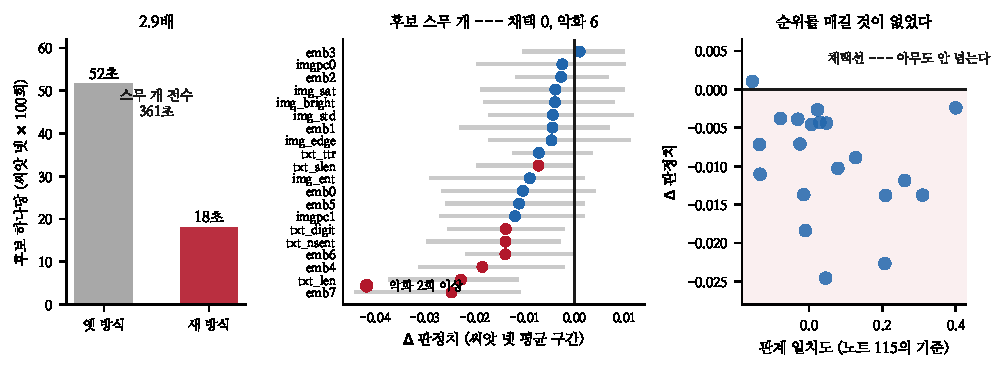
\includegraphics[width=\textwidth]{figs/sw.pdf}
\caption{왼쪽 --- 후보당 52초가 18초로. 가운데 --- 후보 스무 개 전수 판정.
오른쪽 --- 순위를 매길 것이 없었다.}
\end{figure*}

\section{낭비를 셋 고쳤다}

\begin{table}[t]
\centering\tsize
\caption{무엇이 느렸나.}
\begin{tabular}{ll}
\toprule
후보마다 따로 돌렸다 & 복원추출을 후보 수만큼 되풀이 \\
반복마다 축을 다시 만들었다 & 후보 열은 자료가 안 바뀌면 그대로 \\
설정마다 전부 다시 지었다 & 안 건드린 도메인은 인자 공간이 같다 \\
\bottomrule
\end{tabular}
\end{table}

셋째가 핵심이다. 후보 축 하나를 넣으면 그 축을 받는 도메인만 인자 공간이
바뀐다. 나머지는 \emph{글자 그대로 같은 값}이므로 다시 지을 이유가 없다.

\begin{quote}\fontsize{9.0}{11}\selectfont\ttfamily
python3 -m state.sweep --seeds 4 --reps 100\\[.3em]
\rm state/sweep.py \quad 복원추출 한 번에 후보 전부\\
\rm state/candidates.py \quad 후보 자료를 한 번만 만든다
\end{quote}

\begin{table}[t]
\centering\tsize
\caption{같은 조건 비교. 씨앗 넷 $\times$ 반복 100회 환산.}
\begin{tabular}{lr}
\toprule
옛 방식(후보마다 복원추출, 전부 다시) & 52초 \\
\textbf{새 방식} & \textbf{18초} \\
\midrule
배수 & \textbf{2.9배} \\
\midrule
\textbf{후보 스무 개 전수} & \textbf{361초} \\
\bottomrule
\end{tabular}
\end{table}

\claimx{\textbf{전수 검정이 육 분이면 된다.} 나침반이 필요할 만큼 비싸지
않다.}{2.9배는 구조를 고친 몫이다. 그전의 임시 스크립트들은 후보 자료를
반복마다 다시 만들어 훨씬 느렸는데, 그것은 구현 실수이지 방법의 비용이
아니므로 배수에 안 넣었다.}

\section{채택 0/20}

\begin{table}[t]
\centering\tsize
\caption{후보 스무 개. 씨앗 넷 · 반복 100회.}
\begin{tabular}{lrrl}
\toprule
& $\Delta$ & 악화 & 구간(첫 씨앗) \\
\midrule
emb3 & $+$0.0011 & 0 & $-$0.0108 $\sim$ $+$0.0102 \\
표지 주성분 & $-$0.0024 & 0 & \\
emb2 & $-$0.0026 & 0 & \\
표지 채도 & $-$0.0038 & 0 & \\
$\cdots$ & & & \\
숫자 비율 & $-$0.0137 & \textbf{4} & \\
\textbf{문장 수} & $-$0.0138 & \textbf{4} & \\
emb6 & $-$0.0138 & 2 & \\
emb4 & $-$0.0184 & \textbf{4} & \\
\textbf{설명문 길이} & $-$0.0227 & \textbf{4} & \\
\textbf{emb7} & \textbf{$-$0.0246} & \textbf{4} & $-$0.0438 $\sim$ $-$0.0118 \\
\midrule
\multicolumn{4}{l}{\textbf{채택 0/20 · 악화 여섯}} \\
\bottomrule
\end{tabular}
\end{table}

\claimx{\textbf{후보 스무 개 중 채택이 하나도 없다.} 열아홉이 음수이고 여섯이
씨앗 둘 이상에서 악화다. 가장 나은 emb3 도 $+$0.0011에 구간이
$[-0.011, +0.010]$ 이다.}{후보 스무 개가 전부 설명문 · 표지에서 나온 것이다.
다른 종류의 자료(가격 이력 · 검색량 · 리뷰 텍스트)는 아직 안 긁었다.}

\section{나침반이 세 번 죽은 이유}

\begin{quote}\fontsize{9.5}{11.5}\selectfont
\textbf{순위를 매길 것이 없었다.} 노트 101 · 104 · 115의 세 기준은 후보
스무 개를 줄 세우려 했는데, 스무 개가 전부 못 쓸 것이면 ``정확히 줄 세우는''
기준도 쓸모가 없다. 기준이 나빠서 실패한 것이 아니라 \textbf{고를 것이
없어서} 실패했다.
\end{quote}

\claimx{세 기준의 실패는 기준의 결함이 아니라 \textbf{후보군의 결함}이었다.
노트 115의 관계 일치도와 $\Delta$판정치를 겹쳐 보면 스무 점이 전부 0 아래
좁은 띠에 몰려 있다 --- 어떤 축으로 세워도 순위가 의미를 못 갖는다.}
{그래도 세 기준이 ``이 후보군은 전부 못 쓴다''를 미리 말해 주지는 못했다.
그것을 말해 주는 기준이 있으면 여전히 값을 한다.}

\section{긁는 전략이 바뀐다}

\begin{table}[t]
\centering\tsize
\caption{전과 후.}
\begin{tabular}{ll}
\toprule
전 & 어느 것을 긁을지 고른다(기준이 필요) \\
& $\to$ 긁는다 $\to$ 판정한다(비쌈) \\
\midrule
\textbf{후} & \textbf{싼 것을 다 긁는다} \\
& $\to$ \textbf{다 걸어 본다(육 분)} \\
\bottomrule
\end{tabular}
\end{table}

노트 101이 세운 지침(``긁기 전에 재라'')은 노트 102가 죽였고, 대안을 두 번 더
찾다 실패했다. \textbf{이제 지침이 뒤집힌다 --- 재지 말고 긁어서 걸어 봐라.}
판정이 육 분이면 재는 비용이 걸어 보는 비용보다 크다.

\section{한계}

\begin{itemize}[leftmargin=1.1em,itemsep=0.15em]
\item \textbf{채택할 것이 없다.} 스무 개 전부 못 넘는다.
\item 후보군이 설명문 · 표지에 한정된다. 결론은 ``이 스무 개가 안 된다''이지
      ``새 축이 없다''가 아니다.
\item 2.9배는 구조 개선분이다. 임시 스크립트의 낭비는 뺐다.
\item 반복 100회 · 씨앗 넷은 그대로다. 반복을 줄이면 더 빨라지지만 구간이
      넓어진다.
\item 안 건드린 도메인의 인자 공간을 공유하는 것이 옳으려면 \texttt{lam}
      이 안 바뀌어야 한다. 지금 \texttt{lam} 은 1.0 고정이라(노트 48) 성립한다.
\end{itemize}

\section{다음}

\begin{enumerate}[leftmargin=1.3em,itemsep=0.15em]
\item \textbf{다른 종류를 긁는다} --- 설명문 · 표지가 다 막혔으니 남은 것은
      \emph{시간에 따라 변하는} 자료다. 검색량 · 가격 이력 · 리뷰 수 추이.
      지금 축은 전부 한 시점의 정적 값이다. \textbf{이제 걸어 보는 비용이
      싸므로 대량으로 긁어 다 걸 수 있다.}
\item \textbf{팝업 레코드} --- 열 노트가 같은 곳을 가리킨다.
\item 텀블벅 API --- 펀딩만 미디어 홍보 0\%다.
\item 반복 수와 구간 폭의 교환 --- 반복 40회로 줄여도 판정이 같은지.
\end{enumerate}

\vspace{0.6em}
\hrule height 0.3pt
\vspace{0.5em}
{\footnotesize
\textbf{참고문헌}\\[0.3em]
Efron, B., Tibshirani, R. J. (1993). \emph{An Introduction to the Bootstrap}.
Chapman \& Hall.\\[0.15em]
Guyon, I., Elisseeff, A. (2003). An introduction to variable and feature
selection. \emph{JMLR}, 3, 1157--1182.\\[0.15em]
Cawley, G. C., Talbot, N. L. C. (2010). On over-fitting in model selection and
subsequent selection bias in performance evaluation. \emph{JMLR}, 11, 2079--2107.\\[0.15em]
Schoenemann, P. H. (1966). A generalized solution of the orthogonal Procrustes
problem. \emph{Psychometrika}, 31(1), 1--10.\\[0.15em]
Ben-David, S. et al. (2010). A theory of learning from different domains.
\emph{Machine Learning}, 79(1--2), 151--175.
}

\end{document}
